\begin{figure}[t]
    \centering
\begin{tikzpicture}[line width = 1pt,rounded corners,
arrow/.style={line width = 2.5pt},scale=\normscale,every node/.style={scale=\normscale},font = \large]

\def\spacex{1.0}

\node[draw,fill=servcol,align=left,inner sep=10pt,label={north:\textbf{Server}}] (serv) at (0,0) {\textbf{Feature \#1:} 19 - 41 \\ \textbf{Feature \#2:} 31  - 66};
\node[inner sep=0pt,below = 1.8 of serv] (truck2) {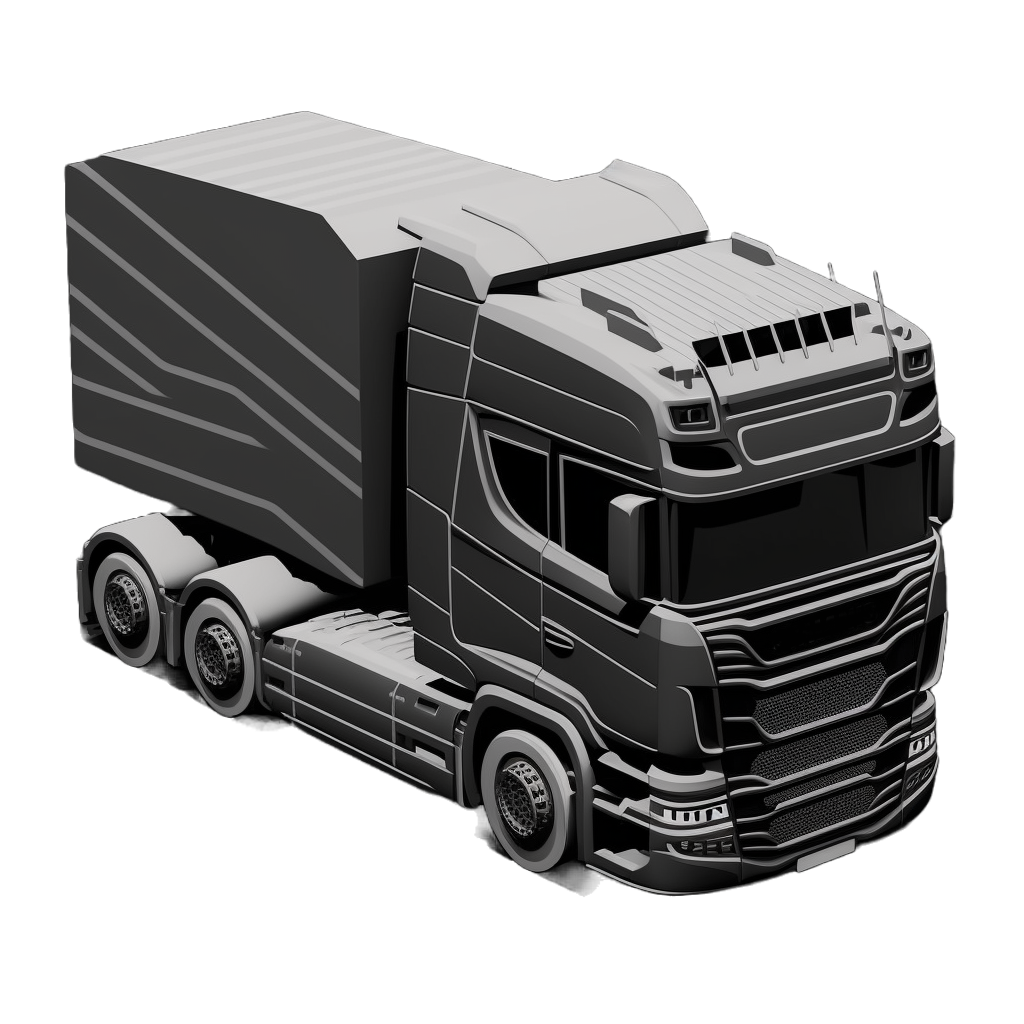
\includegraphics[width=.2\textwidth]{Images/scania-truck.png}};

\node[inner sep=0pt,left = \spacex of truck2] (truck1) {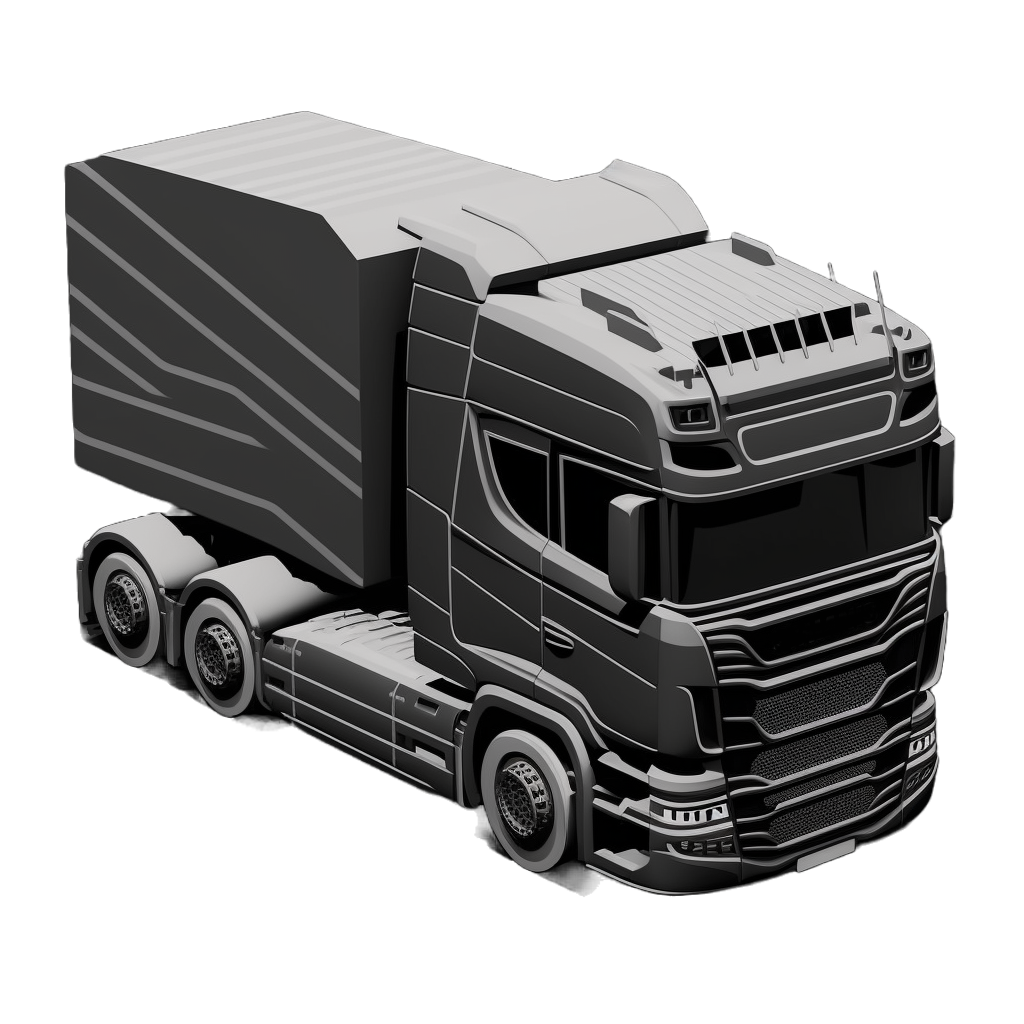
\includegraphics[width=.2\textwidth]{Images/scania-truck.png}};
\node[inner sep=0pt, right = \spacex of truck2] (truck3) {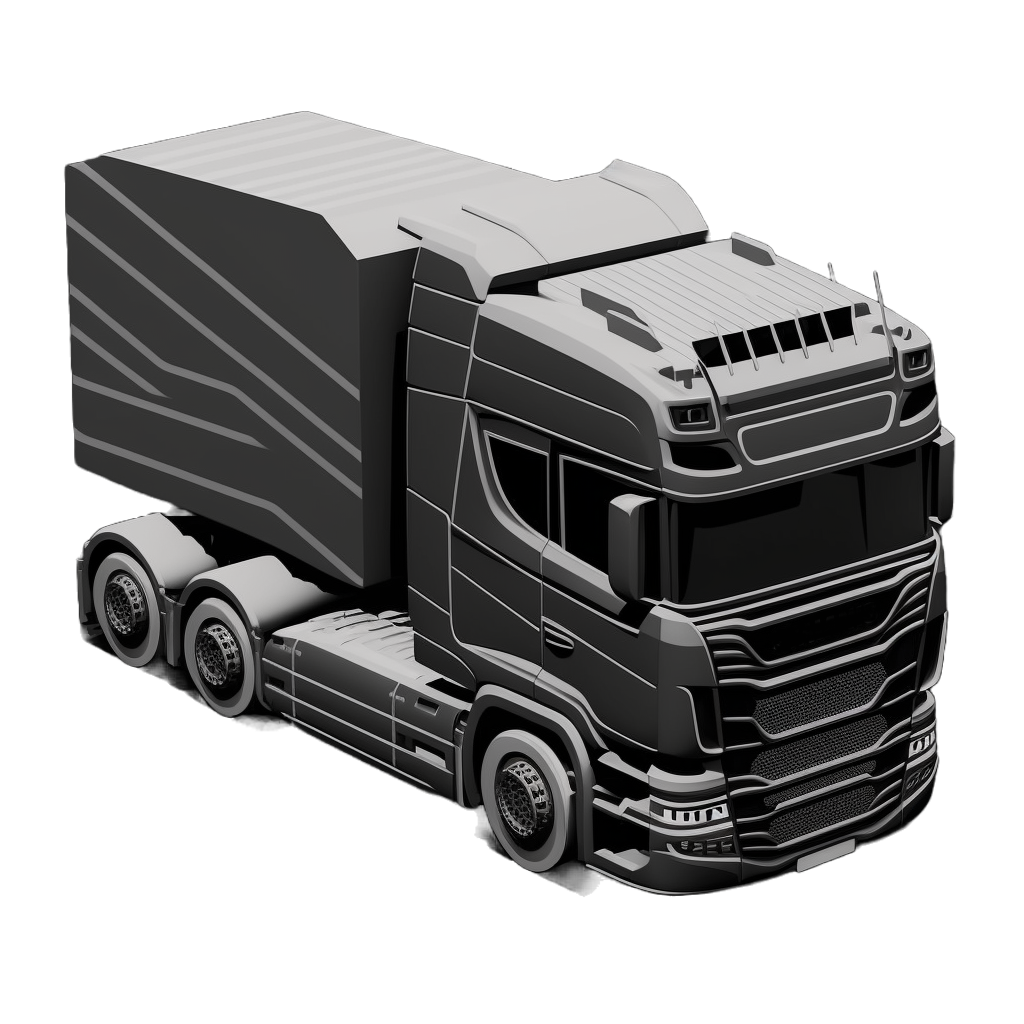
\includegraphics[width=.2\textwidth]{Images/scania-truck.png}};

\node[draw, above left = 0 and 0 of truck1,align=left,anchor = north west,fill=white,fill opacity = 0.7,fill=workcol] (work1) {\textbf{Feature \#1:} 19 - 36 \\ \textbf{Feature \#2:} 45  - 66};

\node[draw, above left = 0 and 0 of truck2,align=left,anchor = north west,fill=white,fill opacity = 0.7,fill=workcol] (work2) {\textbf{Feature \#1:} 23 - 29\\\textbf{Feature \#2:}  31 - 36};


\node[draw, above left = 0 and 0 of truck3,align=left,anchor = north west,fill=white,fill opacity = 0.7,fill=workcol] (work3) {\textbf{Feature \#1:} 26 - 41 \\ \textbf{Feature \#2:} 40 - 55};

\draw[arrow,myred] (serv.180) to [bend right] node[above,sloped,align=center] {19 - 41 \\ 31  - 66} (work1.100);
\draw[arrow] (work1.80) to node[below,sloped,align=center] {19 - 36 \\ 45  - 66} (serv.185);

\draw[arrow,myred] (serv.0) to [bend left] node[above,sloped,align=center] {19 - 41 \\ 31  - 66} (work3.80);
\draw[arrow] (work3.100) to node[below,sloped,align=center] {26 - 41 \\ 40  - 55} (serv.-5);

\draw[arrow] (work2.80) to node[above,sloped,align=center] {23 - 29 \\ 31  - 36} (serv.280);
\draw[arrow,myred] (serv.260) to [bend right] node[above,rotate=180,sloped,align=center] {19 -41 \\ 31 - 66} (work2.100);

\end{tikzpicture}
    \caption{Decentralized data normalization based on workers' minimum and maximum feature values.}
    \label{fig:normalize}
\end{figure}